\documentclass[a4paper,11pt,sf]{leaflet}
%TODO remove notumble
\renewcommand{\familydefault}{\sfdefault}

\usepackage[utf8]{inputenc}
\usepackage[T1]{fontenc}
\usepackage[french]{babel}

\usepackage[official]{eurosym}

\usepackage{graphicx,wrapfig}

\usepackage{url}

\begin{document}

\begin{center}
  \vspace*{\fill}
  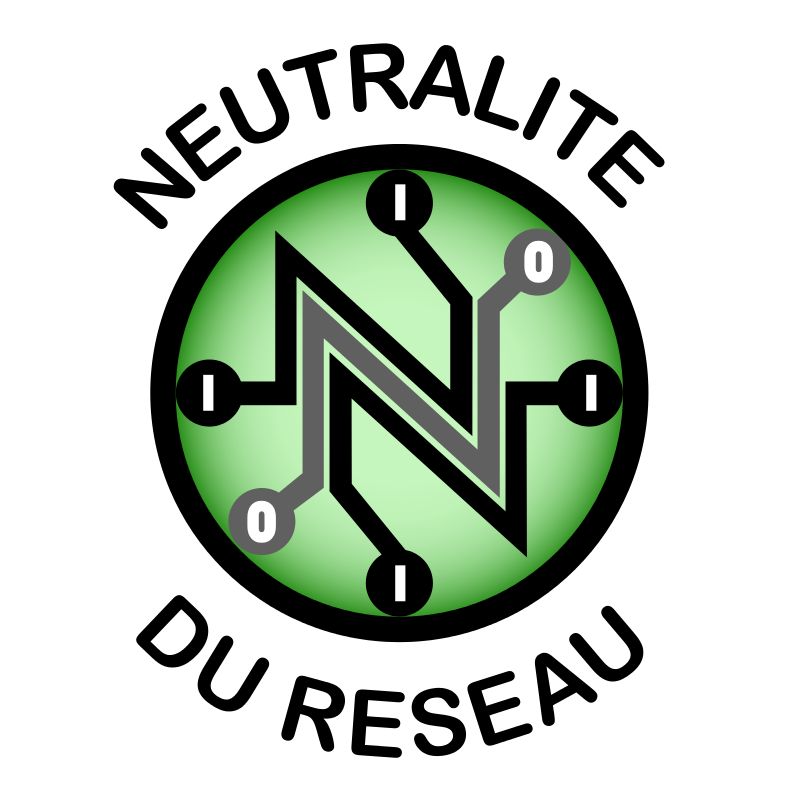
\includegraphics[width=4cm]{neutralite-du-reseau} \\[0.75cm]
  
  \LARGE
  \textbf{La Neutralité du Net}
  \\[2cm]
\end{center}

\section{Qu'est-ce que c'est?}\label{kezako}

La neutralité du Net est un principe fondateur d'Internet qui garantit
que les opérateurs de télécoms ne discriminent pas les communications de
leurs utilisateurs, mais demeurent de simples transmetteurs
d'information. Ceci permet à tous les utilisateurs, quelles que
soient leurs ressources, d'accéder au même réseau dans son entier.

C'est un principe qui est aujourd'hui remise en cause à mesure que les
opérateurs développent des modèles économiques qui restreignent l'accès
à Internet de leurs abonnés, en bridant ou en bloquant l'accès à
certains contenus, services ou applications en ligne (protocoles, sites
web, etc.), ainsi qu'en limitant leur capacité de publication.

Par exemple, sans Neutralité, Facebook pourrait payer les fournisseurs d'accès à internet---tels que Belgacom---pour que leur site web soit plus rapide que les autres.

%En résumé, la neutralité du Net, c'est le fait que les opérateurs
%transmettent les données:
%\begin{itemize}
%\item sans en examiner le contenu, 
%\item sans discriminer la source ou la destination,
%\item sans discriminer le protocole de communication, 
%\item sans en altérer le contenu.
%\end{itemize}

\clearpage
\section{Les arguments pour la neutralité du Net}

\subsection{Neutralité du Net et démocratie}

Contrairement aux moyens traditionnels de communication, tels que la
radiodiffusion ou la télédiffusion, produire et diffuser de
l'information sur internet est relativement peu cher. Cet accès
élargi aux moyens de production et de diffusion de l'information contribue
à rendre plus égalitaire l'accès à la sphère communicationnelle.

La neutralité du Net, en assurant l'égal traitement des flux
d'information, permet de garantir que l'accès au réseau ne dépend pas
des ressources financières des utilisateurs. Acteurs commerciaux et
non-commerciaux sont sur un pied d'égalité. Chacun est libre de
s'exprimer ouvertement, dans les limites fixées par la loi, et d'accéder à
l'information ou aux services qui lui plaisent, que ceux-ci soient payants ou
non. Aussi, l'ensemble des sources d'information disponibles sur
internet représente ainsi une diversité bien plus grande que celle
permise par les médias traditionnels, ce qui constitue un progrès
démocratique notable.

\subsection{Neutralité du Net et innovation}

De même qu'un internet neutre constitue une plate-forme de communication
égalitaire pour la création et la diffusion de messages, tout service ou
innovation peut être librement distribué sur le réseau, quand bien même
il entre en concurrence avec les offres commerciales des opérateurs de
réseaux (exemple du service de téléphonie sur IP Skype).

Le concept d'\og{}innovation sans permis\fg{} --- caractéristique d'internet et
qui permet à des start-ups de distribuer de nouveaux services à moindre
coût et sans accord préalable des opérateurs de réseau --- est au
fondement même du développement d'internet. Or, ce principe est remis en
cause puisque certains fournisseurs d'accès bloquent l'utilisation de
certaines applications, en particulier sur les réseaux internet sans fil
(3G).

\section{Les arguments contre la neutralité du Net}

Les opérateurs de réseau estiment qu'ils doivent être en mesure de gérer
le trafic internet en vue de garantir une qualité de service minimale en
termes de débit et de temps de latence. Cela se traduirait par exemple
par le lancement d'offres d'accès internet \og{}haut de gamme\fg{}, qui
garantiraient aux abonnés un débit minimal, y compris en période de
congestion du réseau. Or, pour garantir de tels débits en période de
congestion, il faudrait nécessairement restreindre l'accès des personnes
n'ayant pas souscrit à cette offre.

Les opérateurs de télécommunications voudraient également tirer parti de
la demande croissante en contenu, dont ils estiment supporter
l'essentiel du coût au travers de leurs investissements dans les
infrastructures, alors que les fournisseurs de contenu tels que Google,
Microsoft ou Skype engrangent d'importantes recettes. Il s'agirait donc
pour les fournisseurs d'accès internet de monétiser l'accès à ces
services. Ces derniers seraient contraints de verser une partie de leurs
revenus aux opérateurs en échange de l'accès au consommateur.

\section{Exemples concrets de remise en cause de la neutralité du Net}

Les atteintes à la neutralité du réseau peuvent être le fait de
discriminations à l'égard de la source, de la destination ou du contenu
de l'information transmise via le réseau.

\subsection{Discrimination à l'égard de la
destination}\label{discrimination-uxe0-luxe9gard-de-la-destination}

Les premières remises en cause de la neutralité du Net sont apparues aux
États-Unis en 2005, avec les déclarations du PDG d'AT\&T, Ed Whitacre,
dénonçant l'utilisation du réseau à titre gratuit par Google et Yahoo.

En 2005, au Canada, l'opérateur Telus a bloqué l'accès vers des sites de
syndicats à l'occasion d'un mouvement social interne. Davantage encore
qu'une atteinte à la neutralité du Net, cette mesure fut dénoncée comme
de la censure.

En 2010, l'opérateur virtuel M6 Mobile utilisant le réseau Orange
annonce une offre à 1 \euro{} par mois ne donnant accès qu'aux pages web
des réseaux sociaux Facebook et Twitter.

\subsection{Discrimination à l'égard du
contenu}\label{discrimination-uxe0-luxe9gard-du-contenu}

En 2007, l'opérateur Comcast, qui possède également de nombreux groupes
de médias, a ralenti le trafic peer-to-peer sur ses réseaux, ce qui lui
valut d'être sanctionné par la Federal Communications Commission, le
régulateur américain des médias et des télécommunications.

En France, les opérateurs proposent des forfaits internet 3G+ qui
bloquent des services Voix sur réseau IP (tel que Skype). Le 13 avril
2010, Orange a annoncé l'autorisation des applications VoIP sur son
réseau, alors que SFR et Bouygues Telecom confirment leur volonté
d'offrir également l'accès à cette technologie.

\subsection{Discrimination à l'égard de la
source}\label{discrimination-uxe0-luxe9gard-de-la-source}

En France, Orange a mis en place en aout 2010 des offres commerciales
internet mobile permettant, moyennant surcoût, d'accéder de façon
illimitée au service de musique en stream Deezer alors que son forfait
mobile est, pour les autres sources de contenus du même type, limité à 1
Go par mois, le rendant inutilisable pour accéder à des services
concurrents.

En France toujours, Bouygues Telecom a créé une offre garantissant un
accès \og{}prioritaire\fg{} sur le reste de ses clients en cas de congestion
du réseau.

\subsection{Altération du contenu}\label{altuxe9ration-du-contenu}

En France, en 2013, il est révélé que SFR recompresse les images et
altère le code de façon à le rendre moins lourd sur son réseau 3G.

Toujours en France, Sosh, la filiale \og{}low cost\fg{} d'Orange, est
suspectée d'injecter dans les pages webs de la version mobile de
Facebook deux liens cliquables (\og{}mes communautés\fg{} et \og{}retour à Orange
World\fg{}) favorisant les services Orange.

\section{Pour aller plus loin}\label{pour-aller-plus-loin}

\subsection{La quadrature du net}\label{la-quadrature-du-net}

\begin{wrapfigure}{l}{0.3\linewidth}

\includegraphics[width=\linewidth]{quadraturenet.png}
\end{wrapfigure}

Au quotidien, La Quadrature du Net agit pour la défense des droits et
libertés des citoyens sur Internet. Cet objectif passe par
l'organisation de campagnes de sensibilisation et de mobilisation, la
publication d'analyses détaillées, le développement d'outils, la
rencontre de décideurs politiques mais aussi des interventions
publiques.

Ils campagnent:
\begin{itemize}
\item pour la défense de la neutralité du Net et la non-discrimination
des données;
\item pour la protection du droit à la vie privée et des données
personnelles;
\item contre la surveillance de masse;
\item pour une réforme positive du droit d'auteur et contre la répression
du partage;
\item pour la défense de la liberté d'expression contre la censure;
\item pour l'exclusion des dispositions concernant nos droits fondamentaux
des accords internationaux;
\item pour la participation citoyenne aux processus démocratiques.
\end{itemize}

\subsection{La FFDN}\label{la-ffdn}

\begin{wrapfigure}{r}{0.3\linewidth}

\includegraphics[width=\linewidth]{ffdn.png}
\end{wrapfigure}

La fédération FDN regroupe des Fournisseurs d'Accès à Internet
associatifs se reconnaissant dans des valeurs communes : bénévolat,
solidarité, fonctionnement démocratique et à but non lucratif; défense
et promotion de la neutralité du Net. À ce titre, la fédération FDN se
donne comme mission de porter la voix de ses membres dans les débats
concernant la liberté d'expression et la neutralité du Net. Elle fournit
à ses membres les outils pour se développer et répondre aux
problématiques qui concernent l'activité de fournisseur d'accès à
Internet.

\section{Sources}\label{sources}

\url{fr.wikipedia.org/wiki/Neutralite_du_reseau}

\url{www.laquadrature.net}

\url{www.ffdn.org}

\vspace*{\fill}
\begin{minipage}{.3\textwidth}
  \centering
  
\includegraphics[width=1.5cm]{llnux} \\
  Louvain-li-Nux
\end{minipage}%
\hfill
\begin{minipage}{0.5\textwidth}
  \hfill
  
\includegraphics[width=4cm]{cc-by-sa}
\end{minipage}

\end{document}
